\documentclass{beamer}
\usetheme{Madrid}
\usecolortheme{beaver}
\usepackage[utf8]{inputenc}
\graphicspath{ {./images/} }

\title{Movie Management System}
\author{ 
        VU1S2223017 - Raj Mayekar\\
        VU1S2223008 - Siddhesh Patil\\
        VU1S2223015 - Afnan Shaikh\\
        VU1S2223018 - Mayuresh Patil
}
\date{SEM III - Miniproject}

\begin{document}

\maketitle  

\begin{frame}
    \frametitle{AGENDA}
    \begin{itemize}
        \item Introduction
        \item Details of Project
        \item Use of project in Real Life
        \item Output
        \item Conclusion
    \end{itemize}
\end{frame}

\begin{frame}{Introduction}
    \begin{itemize}
        \item It is designed to manage the record of movie schedules, movie collection, and ticket sales
                  \vspace{0.5cm}
        \item It Provides a friendly  interface for the user  to enter, retrieve and  manage records through   tables,  forms, queries, and reports.
                  \vspace{0.5cm}
        \item Movie  Management System represents  ticket  booking  and  theater management.
    \end{itemize}
\end{frame}

\begin{frame}{CRUD Operations}
    \begin{itemize}
        \item\textbf {Creation  Of  New  User}
        \\In this Movie Management System, We can create a user and add new movies.
                  \vspace{0.3cm}
        \item\textbf{Read and View the movie reviews and the cast details}
        \\We can read and  view movie reviews and  the movie timings and also  read the cast  details.
                  \vspace{0.3cm}
        \item\textbf{ Update movie shows and their times}
        \\ As an Admin, We can update movie shows and their timings
          \vspace{0.3cm}
        \item\textbf{Delete  or  Cancel  the  Movie  Tickets}
        \\You  As a user, We can  Cancel  the Movie Tickets and  as an Admin We can delete the movies also.
    \end{itemize}
\end{frame}

\begin{frame}{Details Of Project}
    \begin{itemize}
        \item  A  Movie management system is a tool that helps individuals or organizations manage their movie collection. 
                  \vspace{0.5cm}
        \item This can include features such as cataloging and organizing movies by title, director, genre, and other details, as well as tracking information about the movies such as their runtime, release date, and cast members.
                  \vspace{0.5cm}
        \item  Some movie management systems may also allow users to rate and review movies, as well as keep track of which movies they have watched.
    \end{itemize}
\end{frame}

\begin{frame}{Use of Project in Real Life}
    \begin{itemize}
        \item A  Movie management system can help individuals keep track of the movies they own or have borrowed, as well as provide information about each movie such as its runtime, release date, and cast members. 
          \vspace{0.5cm}
        \item This can help users make informed decisions about which movies to watch and keep their collection organized.
          \vspace{0.5cm}
        \item In a Movie production or distribution company, a movie management system can help staff keep track of which movies are in production, which are in post-production, and which are available for release. 
    \end{itemize}
\end{frame}

\begin{frame}{Software/Technologies Used}
    \begin{columns}
        \column{0.5\textwidth}
            \centering
\includegraphics[height=2cm, width=3cm]{flutter.jpg}
            \begin{itemize}
    
                \item Flutter is an open-source mobile application development framework that is used to develop applications for Android and iOS.
                \item Developing a mobile application for a business or organization, such as a retail store, restaurant, or non-profit
            \end{itemize}

        \column{0.5\textwidth}
            \centering
\includegraphics[height=2cm, width=3cm]{firebase.png}
            \begin{itemize}
                \item Firebase is a platform for building mobile and web applications. It offers a number of tools and services that can be used in projects, including cloud storage, and real-time database. 
                \item Storing and syncing data for a real-time, collaborative application.

            \end{itemize}
    \end{columns}
\end{frame}

\begin{frame}{Output of Project}
\begin{columns}
    \column{0.3\textwidth}
    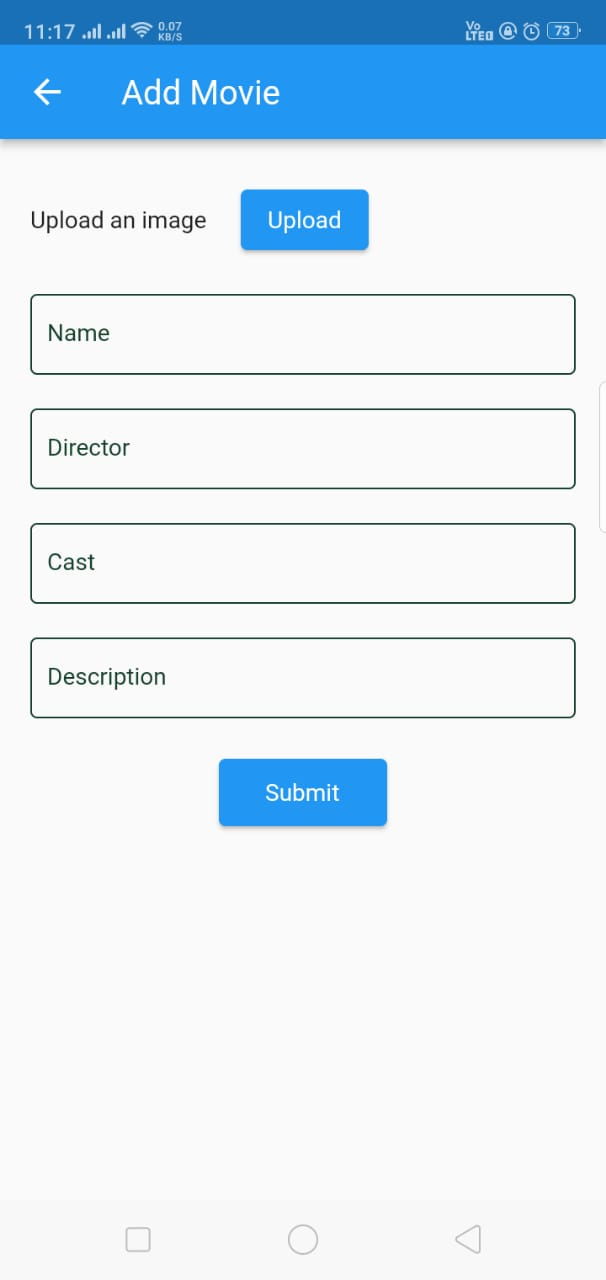
\includegraphics[width=3cm, height=6cm]{ot1.jpeg}
    
    \column{0.3\textwidth}
    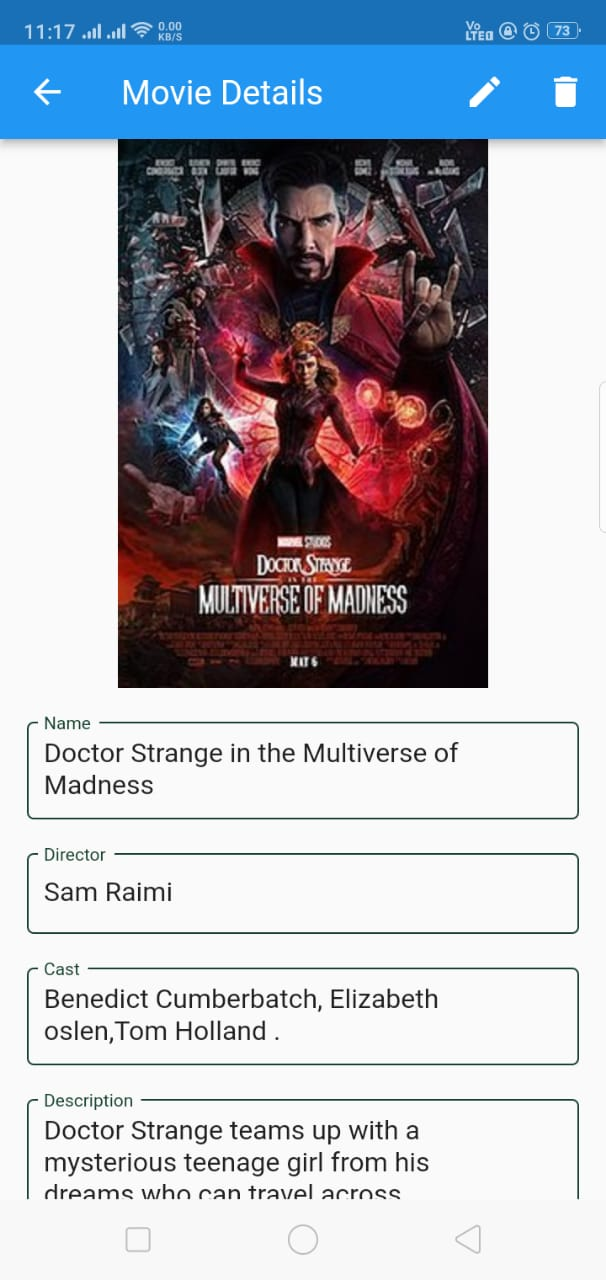
\includegraphics[width=3cm, height=6cm]{ot2.jpeg}
    
    \column{0.3\textwidth}
    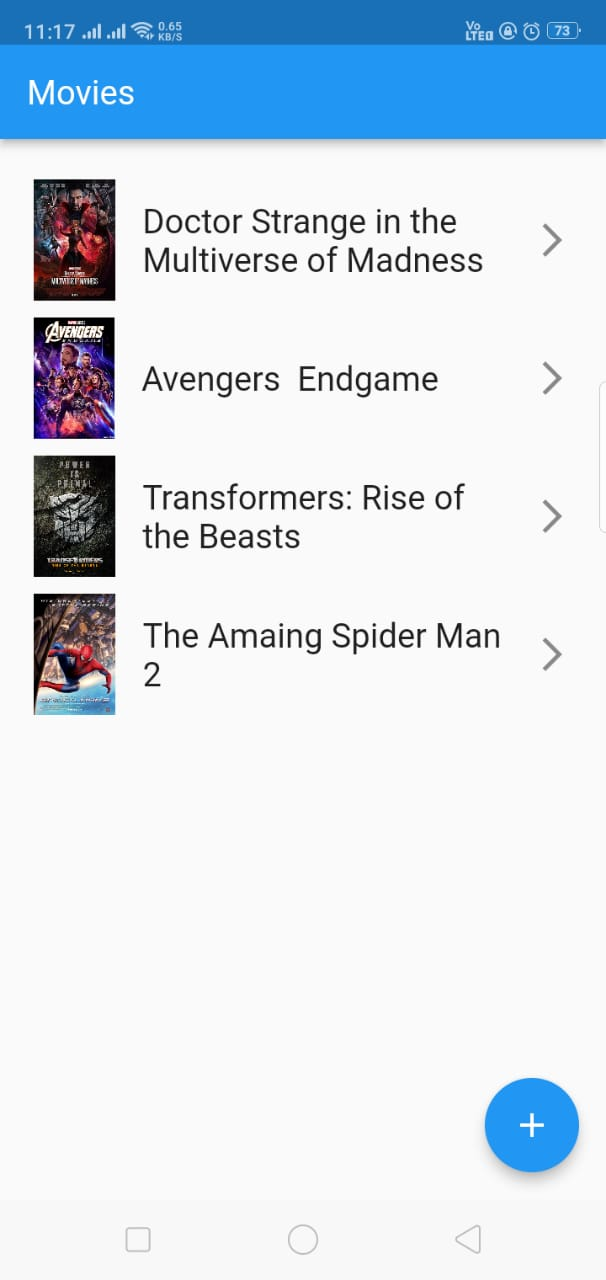
\includegraphics[width=3cm, height=6cm]{ot3.jpeg}
    
\end{columns}
\end{frame}

\begin{frame}
    \vspace{2cm}
    \centering\huge{THANK YOU!!!}
    \vspace{1cm}
    \normalsize {
        \\VU1S2223017 - Raj Mayekar
        \\VU1S2223008 - Siddhesh Patil
        \\VU1S2223015 - Afnan Shaikh
        \\VU1S2223018 - Mayuresh Patil
    }
\end{frame}

\end{document}
